\chapter{Настройка оптического интерферометра методами машинного обучения с подкреплением}\label{ch:ch2}

\section{Физические принципы работы и модель оптического интерферометра}\label{sec:ch2/sec1}

\subsection{Математическая модель интерференции света}\label{sec:ch2/sec1/subsec1}

Работа оптического интерферометра основана на принципе интерференции света --- физического процесса при котором два когерентных световых пучка накладываются друг на друга и образуют в пространстве периодическую структуру состоящую из минимумов и максимумов интенсивности получившую название интерференционной картины. 

\begin{figure}[ht]
    \centerfloat{
        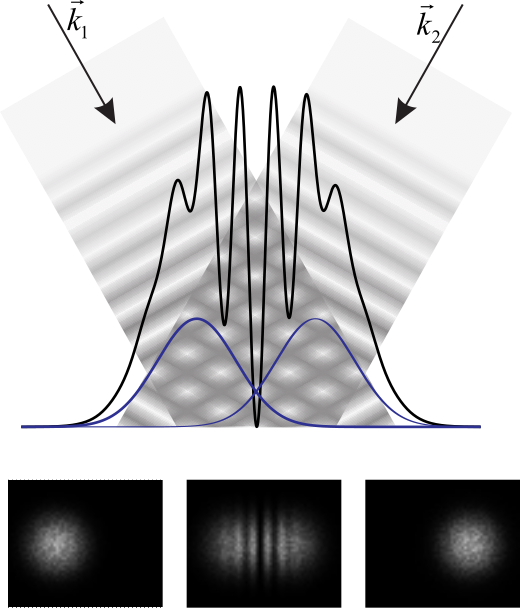
\includegraphics[scale=1.7]{images/interf_expl.png}
    }
    \caption{Одномерный срез интерференционной картины полученный при неполном перекрытии двух когерентных лазерных лучей с волновыми векторами $k_1$ и $k_2$. Волновые фронты показаны с помощью градиента; голубые линии показывают интенсивности индивидуальных лучей (не в масштабе); черные линии соответствуют профилю интенсивности результирующей картины. Соответствующие двумерные изображения индивидуальных лучей и их интерференционной картины представлены внизу.}\label{fig:two_beam_interf}
\end{figure}

Интерференционная картина получаемая при наложении двух когерентных лучей изображена на рис. \ref{fig:two_beam_interf}. Для вычисления интерференционной картины опишем математическую модель интерференции. Рассмотрим световой пучок распространяющийся вдоль оси $z$ в параксиальном приближении $k_z \gg k_x, k_y$, где волновой вектор $\vec{k}$ --- вектор, направление которого перпендикулярно фазовому фронту волны, а абсолютное значение равно волновому числу. Волновое число $k$ связано с длинной волны $\lambda$ соотношением 

\begin{equation*}
    k = \frac{2\pi}{\lambda}
\end{equation*}

Распределение амплитуды излучения будем описывать с помощью нормального распределения. Определим радиус пучка $r$ как расстояние от центра пучка на котором напряженность электромагнитного поля падает в $e$ раз. 
Тогда распределение напряженности электромагнитного поля в каждом световом пучке $E(x, y, z)$ задается следующим выражением: 

\begin{equation}
    E(x,y,z) = e^{-\frac{(x-x_0(z))^2+(y-y_0(z))^2}{r^2}} e^{i k_xx+ik_yy+ik_zz}    
\label{eq:Exyzt}
\end{equation}

где $(x,y,z)$ координатный вектор, $(x_0(z),y_0(z))$ положение центра пучка, $\vec{k}$ волновой вектор $r$ радиус пучка. %We neglect the beam divergence due to diffraction.
Первый множитель уравнения \ref{eq:Exyzt} соответствует амплитуде электромагнитной волны $A(x,y,z)$, а второй --- фазе $\exp(i\phi(x,y,z))$. 
При сложении двух электромагнитных волн в точке $x, y, z$ итоговая напряженность поля будет равна сумме напряженностей отдельных волн: 

\begin{equation}
    E(x, y, z) = E_1(x, y, z) + E_2(x, y, z)
\label{eq:E1E2}
\end{equation}

Видимая интерференционная картина определяется распределением интенсивности света, которая равна квадрату модуля напряженности электромагнитного поля: 

\begin{equation}
    I(x, y, z) = |E(x, y, z)|^2 = E(x,y,z) E^*(x,y,z)
\label{eq:ie2}
\end{equation}

Таким образом в соответствии с уравнениями \ref{eq:Exyzt}, \ref{eq:E1E2}, \ref{eq:ie2} интенсивность света в точке $x, y, z$ сложении двух световых лучей определятся выражением: 

\begin{multline}
    I(x, y, z) = E_1E_1^* + E_2E_2^* + E_1E_2^* + E_2E_1^* = \\
    I_1(x,y,z) + I_2(x,y,z) + 2 \sqrt{I_1(x,y,z)I_2(x,y,z)}\cos(\Delta \phi)
\label{eq:interf}
\end{multline}

где $\Delta \phi = \phi_1 - \phi_2$ --- разность фаз двух волн. Из уравнения \ref{eq:interf} следует, что если две волны складываются синфазно т.е. $\Delta \phi = 0$, то интенсивность света максимальна $I = I_1 + I_2 + 2\sqrt{I_1I_2}$. Если же две волны складываются в противофазе т.е. $\Delta \phi = \pi$, то интенсивность света минимальна $I = I_1 + I_2 - 2\sqrt{I_1I_2}$.

\subsection{Математическая модель интерферометра Маха-Цендера}\label{sec:ch2/sec1/subsec2}

Интерферометры являются одними из основных инструментов в экспериментальной оптике и служат для прецизионного измерения разности фаз между двумя лучами. Интерферометр Фабри-Перо\cite{fabry-perot1899} используется в оптической спектрометрии; интерферометр Майкельсона является основной частью современных детекторов гравитационных волн LIGO и VIRGO \cite{LIGO, VIRGO} он также используется для измерения шероховатости поверхностей; интерферометр Саньяка используется в современных навигационных системах; интерферометр Маха-Цендера является основным инструментом в современных экспериментах в квантовой оптике \cite{Sarkar2006, Sychev2017}. 

В рамках данной работы рассматривалась настройка оптического интерферометра Маха-Цендера методами машинного обучения с подкреплением. Схема работы интерферометра Маха-Цендера изображена на рис. \ref{fig:MZI}. 

\begin{figure}[ht]
\centerfloat{
    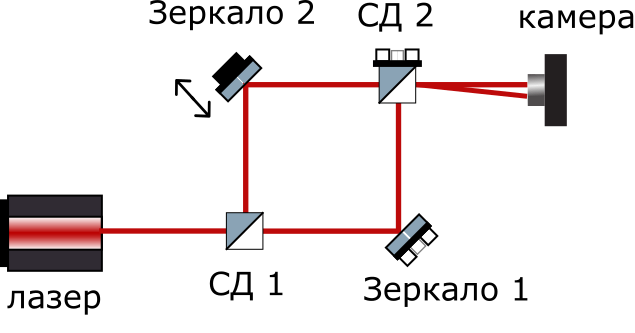
\includegraphics[scale=2.0]{images/MZI_expl.png}
}
\caption{Принципиальная схема работы интерферометра Маха-Цендера}
\label{fig:MZI}
\end{figure}

В ней лазерный луч после прохождения светоделителя СД 1 разделяется на два луча. Верхний луч проходит через зеркало 2 и светоделитель СД 2 и попадает на камеру. Нижний луч проходит через светоделитель СД 1 и зеркало 1. Для настройки интерферометра необходимо точно совместить два луча как по положению, так и по направлению на камере. Регулировка нижнего луча производится с помощью зеркала 1 и светоделителя СД 2. Верхний луч является неподвижным. Настройка интерферометра представляет собой итеративный процесс в котором человек ориентируясь на интерференционную картину, получаемую на камере подстраивает положение зеркала 1 и светоделителя 2, чтобы добиться идеального совпадения лучей. Для визуализации разности фаз между двумя плечами интерферометра зеркало 2 совершает колебательные движения на расстояние порядка длины волны $\lambda$ благодаря чему фаза верхнего луча изменяется в интервале $\phi \in [0, 2\pi)$. Настройка интерферометра представляет собой трудоемкий процесс осложненный тем, что и зеркало 1 и светоделитель СД 2 меняют одновременно и положение луча на камере и угол между лучами. 

\begin{figure}[ht]
\centerfloat{
    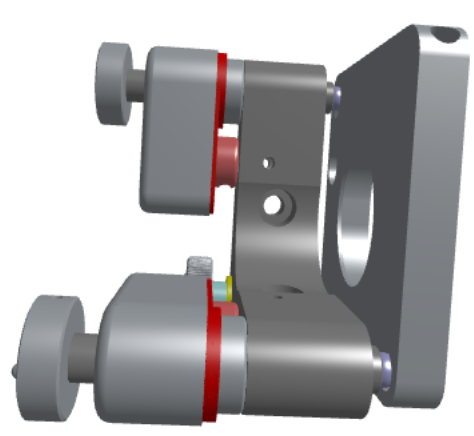
\includegraphics[scale=0.3]{images/mirror_mount.png}
}
\caption{3D модель крепления оптического зеркала использованного в работе \cite{newport_mirror}}
\label{fig:mirror}
\end{figure}

На рис. \ref{fig:mirror} показана 3D модель крепления оптического зеркала использованная в работе для регулировки положения зеркала 1 и светоделителя СД 2. Крепление оборудовано двумя микрометрическими винтами которые также могут управляться с помощью встроенных пьезо двигателей. Каждый из винтов поворачивает зеркало вокруг перпендикулярных плоскостей. Направление вектора нормали зеркала $\vec{n}$ зависит от положений винтов $x, y$ в приближении малых углов следующим образом: 

\begin{equation}
    \vec{n} = \begin{pmatrix}
        x\\ 
        y\\ 
        \sqrt{1 - x^2 - y^2}
    \end{pmatrix}
\end{equation}


Для вычисления интерференционной картины по формуле \ref{eq:interf} необходимо знать положение центров лучей на камере и их фазы. Предполагаем, что верхний луч распространяется точно вдоль оси  $z$, таким образом для него $x_0\equiv y_0\equiv k_x\equiv k_y\equiv 0$. Для нижнего луча в работе производится трассировка нижнего луча через систему зеркал. Введем систему координат с центром в камере как показано на рис. \ref{fig:MZI_coordis}. 


\begin{figure}[ht]
\centerfloat{
    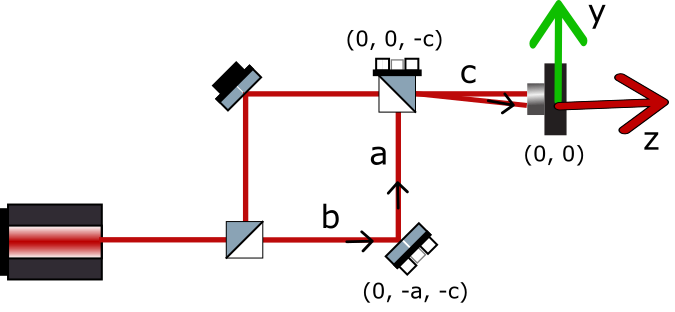
\includegraphics[scale=2.0]{images/MZI_matmodel.png}
}
\caption{Система координат}
\label{fig:MZI_coordis}
\end{figure}

При прохождении каждого зеркала находится точка пересечения луча с плоскостью зеркала и рассчитывается угол поворота луча. Луч вращается относительно плоскости перпендикулярной плоскости образованной вектором нормали зеркала и первоначальным направлением луча. Величина угла определяется из закона отражения. Листинг функции трассировки приведен в приложении \ref{lst:beam_trace}.


\subsection{Видность интерференционной картины}\label{sec:ch2/sec1/subsec3}

Интенсивность интерференционной картины получаемой при наложении двух лучей в плоскости камеры ($z=0$) задается выражением:

\begin{equation}
    I(x,y,t)=|E_1(x,y,0)+E_2(x,y,0)e^{i\phi_{\mathrm{piezo}}(t)}|^2  
\label{eq:I_def}
\end{equation}

где $\phi_{\mathrm{piezo}}(t)$ фазовый сдвиг получаемый из-за движения пьезо зеркала. Таким образом разность фаз $\Delta \phi$ в уравнении \ref{eq:interf} за один проход пьезо зеркала пробегает интервал от $0$ до $2\pi$. Суммарной интенсивностью интерференционной картины называется величина: 

\begin{equation}
    I_{\mathrm{tot}}(t) = \iint_{-\infty}^{+\infty} I(x, y, t) {\mathrm{d}}x{\mathrm{d}}y
\end{equation}

Периодическое движение пьезо зеркала приводит к периодическому изменению суммарной интенсивности. Пример изменения интенсивности интерференционной картины показан на рис. \ref{fig:intens_plot}.

\begin{figure}[ht]
\centerfloat{
    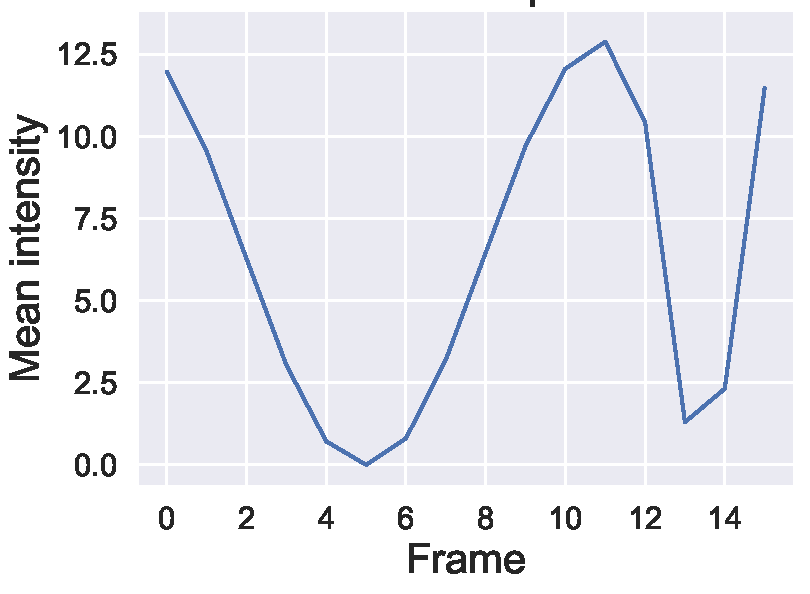
\includegraphics[scale=0.7]{images/piezo_intens_plot.pdf}
}
\caption{График изменения интенсивности (слева) и график движения пьезо зеркала (справа) TODO}
\label{fig:intens_plot}
\end{figure}

Основным критерием качества настройки интерферометра является видность интерференционной картины: 

\begin{equation}
    V = \frac{            
        \max_{t}(I_{\mathrm{tot}}) - \min_t(I_{\mathrm{tot}})}
        {\max_{t}(I_{\mathrm{tot}}) + \min_t(I_{\mathrm{tot}})}
    \label{eq:visib}
\end{equation}

Видность интерференционной картины вычисляется с помощью минимума $\min_t(I_{\mathrm{tot}})$ и максимума $\max_t(I_{\mathrm{tot}})$ суммарной интенсивности света на камере. Максимум и минимум вычисляются за один полный период прохода пьезо зеркала. По определению видность является действительным числом и находится в интервале $V \in [0, 1]$. 

Примеры интерференционных картин и графики соответствующих им суммарных интенсивностей приведены на рис. \ref{fig:visib_expl}. Для полностью настроенного интерферометра [рис.~\ref{fig:visib_expl}(a)], $\min_t(I_{\mathrm{tot}})=0$, таким образом видность $V=1$, для полностью расстроенного интерферометра [Fig.~\ref{fig:visib_expl}(c)], $\min_t(I_{\mathrm{tot}})\approx\max_t(I_{\mathrm{tot}})$, таким образом видность $V\approx 0$.

\begin{figure}[ht]
\centerfloat{
    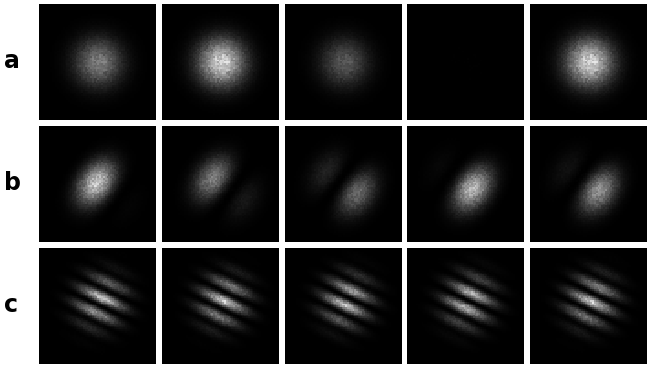
\includegraphics[scale=0.7]{images/visib_expl.png}
}
\caption{Примеры интерференционных картин полученные в симуляции. (a) Полностью настроенный интерферометр, видность = 1; (b) Слабо расстроенный интерферометр, видность = 0.3; (c) Сильно расстроенный интерферометр, видность =
0.0026. Изображения слева на право соответствуют различной разности фаз [$\phi_{\mathrm{piezo}}(t)$] между двумя плечами интерферометра из-за движения пьезо зеркала}
\label{fig:visib_expl}
\end{figure}


Из уравнений.~\eqref{eq:Exyzt} и \eqref{eq:visib}, получим точное выражение для видности интерференционной картины:

\begin{equation}
    V = \exp\left(- \frac{x_0^2 + y_0^2}{2 r^2}\right)  \exp\left[- \frac{(k_x^2 + k_y^2) r^2}{8}\right],
    \label{eq:visib_rot}
\end{equation}

где $x_0$ и $y_0$ координаты центра нижнего луча на камере; $k_x$ и $k_y$ компоненты волнового вектора нижнего луча. Вывод уравнения \ref{eq:visib_rot} приведен в приложении \ref{app:B1}.

\subsection{Математическая модель интерферометра Маха-Цендера с линзами}\label{sec:ch2/sec1/subsec4}

Интерферометр Маха-Цендера показанный на рис.~\ref{fig:MZI} позволяет управлять положением луча на экране и его направлением. Однако он не позволяет управлять его волновым фронтом. Для этого как показано на рис.~\ref{fig:MZI_expl_lenses} в нижнее плечо интерферометра добавляют две собирающие линзы установленные по схеме телескопа т.е. с расстоянием между ними равным суммам их фокусных расстояний. 

\begin{figure}[ht]
\centerfloat{
    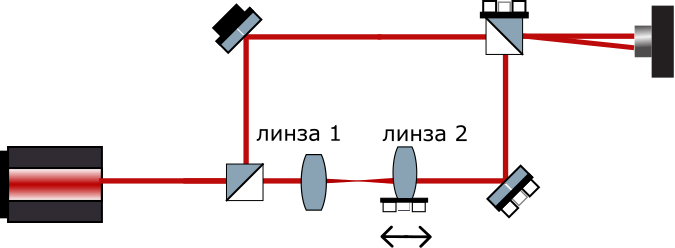
\includegraphics[scale=2.0]{images/MZI_expl_lenses.png}
}
\caption{Схема интерферометра Маха-Цендера с линзами}
\label{fig:MZI_expl_lenses}
\end{figure}

Таким образом помимо зеркала 1 и светоделителя СД 2 настраивать еще нужно положение линзы 2. Положение линзы 2 регулируется с помощью подвижки изображенной на рис.~\ref{fig:lense_mount}. 

\begin{figure}[ht]
\centerfloat{
    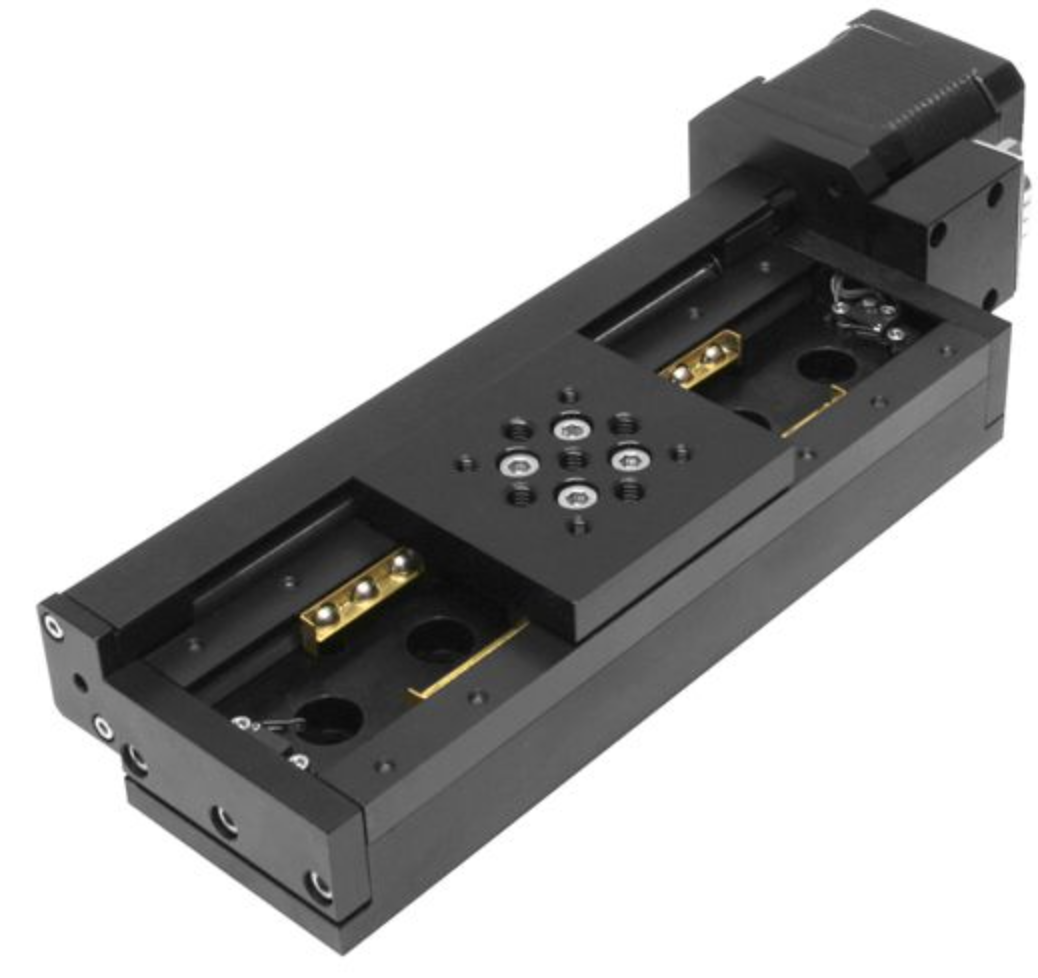
\includegraphics[scale=0.3]{images/lense_mount.png}
}
\caption{Подвижка регулирующая положение линзы 2 в эксперименте \cite{standa_stage}}
\label{fig:lense_mount}
\end{figure}

Лазерные пучки в верхнем и нижнем плечах интерферометра описываются гауссовым поперечным профилем. Напряженность поля в точке с координатами $(x,y,z)$ задается следующим образом: 

\begin{subequations}\label{beams}
\begin{equation}
    E_u={\mathrm{Re}}\left[\exp \left(-\frac{x^{2}+y^{2}}{r_u^{2}(z)}\right) \exp \left(-i\left(k_{z} z+ k\frac{x^2+y^2}{2\rho^2_u(z)} + \phi_{\mathrm{piezo}}(t)\right)\right)\right]
    \label{eq:upper_beam}
\end{equation}
\begin{equation}
    \label{eq:lower_beam}
    \begin{split}
        E_l={\mathrm{Re}}\left[\exp \left(-\frac{\left(x-x_{0}\right)^{2}+\left(y-y_{0}\right)^{2}}{r_l^{2}(z)}\right)  
        \exp \left(-i\left(k_{x} x+k_{y} y+k_{z} z + k\frac{x^2+y^2}{2\rho^2_l(z)} z\right)\right)\right]
    \end{split}
    \end{equation}
\end{subequations}

где индексы $u$ и $l$ соответствуют верхнему и нижнему лучам, $(x_0, y_0)$ положение центра нижнего луча [верхний луч считается центрированным в $(x,y)=(0,0)$], $z$ направление распространения лучей, 
$r(z)$ радиус луча, $\rho(z)$ радиус кривизны волнового фронта, $(k_x,k_y,k_z)$ волновой вектор $k=\sqrt{k_x^2+k_y^2+k_z^2}=2\pi/\lambda$, $\phi_{\mathrm{piezo}}(t)$ фазовый сдвиг из-за движения пьезо зеркала. Также используется параксиальное приближение $k_z \gg k_x, k_y$. 

В отличие от уравнения \ref{eq:Exyzt} в уравнениях \ref{eq:upper_beam} и \ref{eq:lower_beam} волновой фронт уже не является плоским и поэтому рассматривается зависимость радиуса пучка от расстояния $r(z)$ и вводится радиус кривизны волнового фронта $\rho(z)$.

Для моделирования параметров пучка после прохождения системы линз воспользуемся матричным методом \cite{gerrard2012introduction}. В этом методе световой луч характеризуется комплексно значным параметром $q$:

\begin{equation}
    \dfrac{1}{q} = \dfrac{1}{\rho} - \dfrac{i \lambda}{\pi r^2}   
\end{equation}

Преобразования происходящие с лучом при прохождении оптических элементов описываются четырьмя параметрами $ABCD$: 

\begin{equation}
    q^{\prime}=\dfrac{A q+B}{C q+D}   
\end{equation}

Параметры $ABCD$ могут быть записаны в виде матрицы. Для пустого пространства длинны $d$ $ABCD$-матрица имеет вид: 

\begin{equation}
    \begin{bmatrix} A & B \\ C & D \end{bmatrix}=\begin{bmatrix} 1 & d \\ 0 & 1 \end{bmatrix}
\end{equation}

Для линзы с фокусным расстоянием $f$ $ABCD$-матрица имеет вид: 

\begin{equation}
    \begin{bmatrix} A & B \\ C & D \end{bmatrix}=\begin{bmatrix} 1 & 0 \\ -1/f & 1 \end{bmatrix}
\end{equation}

Таким образом для нахождения параметров пучка после прохождения интерферометра помимо трассировки луча требуется еще вычислить его параметры с помощью $ABCD$-матриц. Листинг функции вычисляющей парамеры пучка приведен в приложении \ref{lst:beam_propag}.

\subsection{Видность интерференционной картины в интерферометре Маха-Цендера с линзами}\label{sec:ch2/sec1/subsec5}

Для получения аналитической зависимости видности интерференционной картины в интерферометре Маха-Цендера с линзами нужно вычислить перпендикулярные профили пучков  (\ref{beams}) и рассчитать видность в соответствии с уравнениями \ref{eq:I_def}, \ref{eq:visib}. Итоговое выражение для видности интерференционной картины выглядит следующим образом:

\begin{equation}
\begin{split}
    V =\frac{4}{\left(n^{2}+1\right) r_{\mathrm{upper}}^{2}} \frac{1}{c} \exp \left(-\left(x_{0}^{2}+y_{0}^{2}\right)\left(\frac{1}{r_{\mathrm{upper}}^{2} n^{2}}-\frac{n^{2}+1}{n^{6} r_{\mathrm{upper}}^{6} c^{2}}\right)\right) \times \\ \times \exp \left(-\frac{n^{2}+1}{4 c^{2} n^{2} r_{\mathrm{upper}}^{2}}\left(k_{x}^{2}+k_{y}^{2}\right)\right) \exp \left(\frac{\frac{\pi}{\lambda \rho^{\prime}}}{n^{2} r_{\mathrm{upper}}^{2} c^{2}}\left(x_{0} k_{x}+y_{0} k_{y}\right)\right),
\end{split}
\label{eq:visib_lense}
\end{equation}
где параметр $n=\dfrac{r_{\mathrm{lower}}}{r_{\mathrm{upper}}}$ и параметр $c^2 = (\dfrac{n^2 + 1}{n^2r^2_{\mathrm{upper}}})^2$.

Можно показать, что в случае когда $r_{\mathrm{upper}} = r_{\mathrm{lower}}$, $\rho^{\prime} = \rho = \infty$ формула \ref{eq:visib_lense} совпадает с формулой \ref{eq:visib_rot}. Полный вывод формулы \ref{eq:visib_lense} приведен в приложении \ref{app:B2}.

Примеры интерференционных картин получаемые в интерферометре Маха-Цендера с линзами приведены на рис.~\ref{fig:visib_lens_expl}. Закругленная форма интерференционных полос появляется в следствии интерференции пучков с различной расходимостью. Мы прикладываем ассиметричной пилообразное напряжение к пьезо зеркалу для наблюдения временной динамики интерференционных полос. Амплитуда движения пьезо зеркала соответствует разности фаз пучков порядка $2\pi$. Для расстроенного интерферометра, движение пьезо зеркала приводи к поперечному смещению интерференционных полос как показано на рис. \ref{fig:visib_lens_expl} (b-d), что позволяет извлечь информацию о знаке угла между интерферирующими лучами. В случае если интерферометр полностью настроен, интерференция будет выглядеть как мигающее пятно [рис. \ref{fig:visib_lens_expl} (a)].

\begin{figure}[ht]
\centerfloat{
    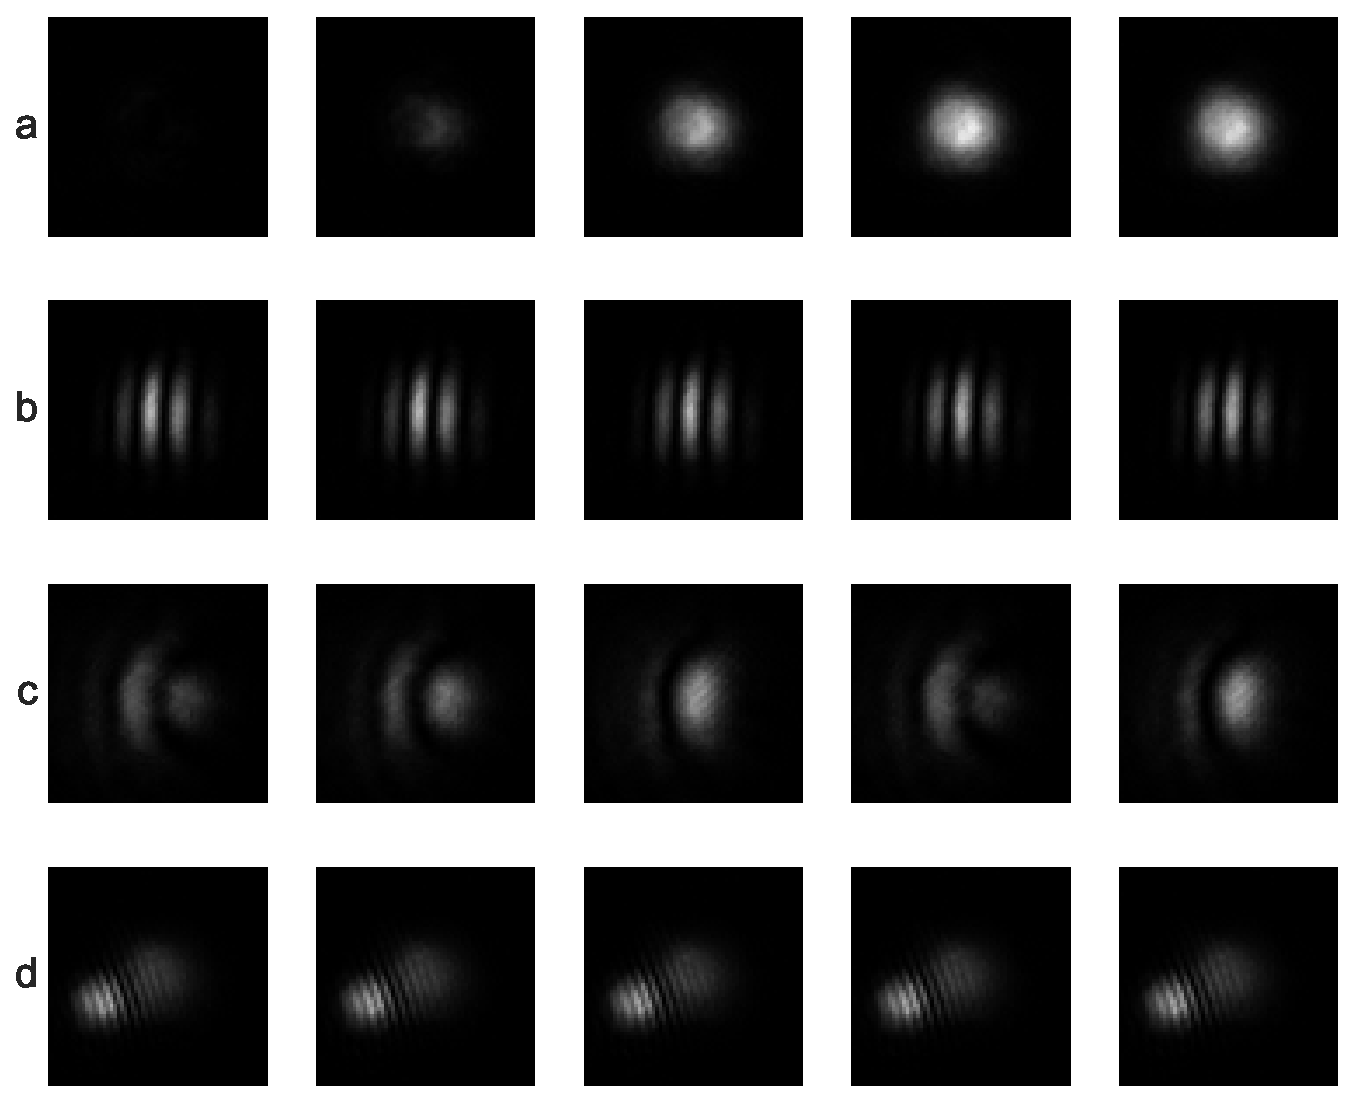
\includegraphics[scale=0.7]{images/Env_patterns.pdf}
}
\caption{Примеры интерференционных картин полученные на интерферометре Маха-Цендена с линзами. (b-d) Пример интерференционных изображений полученных при расстроенном интерферометре. Изображения в каждом столбце соответствуют различным положениям пьезо зеркала.}
\label{fig:visib_lens_expl}
\end{figure}

\subsection{Численная модель интерферометра Маха-Цендера}\label{sec:ch2/sec1/subsec6}

При вычислении интерференционной картины трассировка центра пучка и вычисление его радиуса и кривизны волнового фронта производится согласно описанию в разделах \ref{sec:ch2/sec1/subsec2}, \ref{sec:ch2/sec1/subsec4}. Основная вычислительная сложность состоит в вычислении изображения интерференционной картины согласно ур.~\ref{eq:interf}. Изображение интерференционной картины будем вычислять на равномерной сетке размером $64\times64$ пикселя. За время одного прохода пьезо зеркала будем вычислять 16 интерференционных картин соответствующих различным положениям пьезо зеркала $\phi_{\mathrm{piezo}}(t)$ взятым через одинаковые промежутки времени. 

Вычисление интерференционной картины схематически показано на рис.~\ref{fig:wave_front_projection}. Алгоритм вычисления интерференционной картины \ref{alg:interf_img_calc} проецирует две волны на пиксели камеры и в каждом пикселе считает интенсивность результирующей волны согласно ур.~\ref{eq:I_def}. 

\begin{figure}[ht]
\centerfloat{
    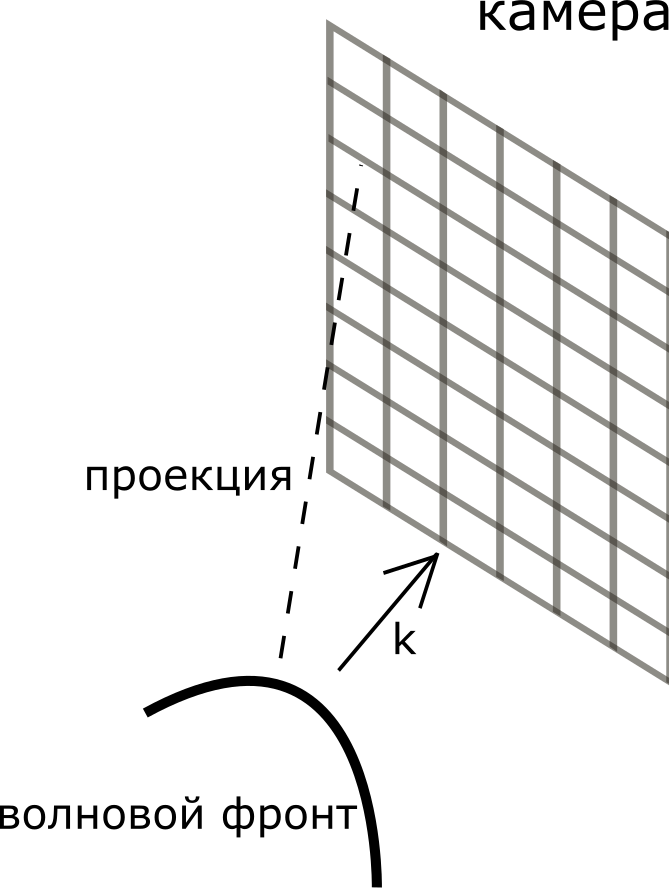
\includegraphics[scale=0.4]{images/wave_front_projection.png}
}
\caption{Вычисление интерференционной картины}
\label{fig:wave_front_projection}
\end{figure}

\begin{algorithm}[ht]
	\SetAlgoLined
	\KwIn{$r_1, r_2$ - радиус $\rho_1, \rho_2$ - радиус кривизны, $(x,y)_1, (x,y)_2$ - координаты центра, $\vec{k}_1,\vec{k}_2$ - k-вектор, $N_{\mathrm{frames}}$ - число шагов по времени, $N_{\mathrm{pixels}}$ - число пикселей}
	\KwOut{image - 2d array}
	\ForEach{frame in $\{1...N_{\mathrm{frames}}\}$}{
	    \ForEach{pixel in $\{1...N_{\mathrm{pixels}}\}$}{
	        // найдем ортогональную проекцию пикселя на волновой фронт\;
            source1 = backTrack(pixel, $k_1$, $x_1$, $y_1$)\;
            source2 = backTrack(pixel, $k_2$, $x_2$, $y_2$)\;

	        // найдем расстояние пройденое лучом\;
	        dist1 = dist(pixel, source1)\; 
	        dist1 = dist(pixel, source2)\; 

	        // рассчитаем амплитуду и фазу волны\;
	        w1 = calcWave(dist1, source1, $\rho_1$)\;
	        w2 = calcWave(dist2, source2, $\rho_2$)\;

	        // рассчитаем интенcивность света\;
	        image[pixel] = intens(w1, w2)\;
	    }
	}
\caption{Алгоритм вычисления интерференционной картины}
\label{alg:interf_img_calc}
\end{algorithm}


\section{Настройка оптического интерферометра как задача машинного обучения с подкреплением}\label{sec:ch2/sect2}

Рассмотрим более детально процесс настройки оптического интерферометра Маха-Цендера. Настройка представляет собой итеративный процесс в котором человек подстраивает положения зеркал и линз в зависимости от текущей интерференционной картины наблюдаемой на камере. Отличительной особенностью настройки интерферометра является, необходимость получить значение видности как можно ближе к $1$. Это приводит к тому, что по мере приближения видности к $1$ требуется совершать действия все меньшего размера. Несмотря на то, что истинное состояние интерферометра (положение зеркал, и линз) для человека недоступно информации получаемой из видео потока (размер интерференционных полос, их ориентация, их направление движения) в целом достаточно, чтобы понять в какую сторону и примерно на сколько следует повернуть управляющие элементы зеркал. Интерференционную картину можно рассматривать как отображение из $n$-мерного пространства состояний ($\mathcal{R}^4$ для интерферометра с двумя зеркалами, $\mathcal{R}^5$ для интерферометра с двумя зеркалами и одной подвижной линзой) в пространство наблюдений --- двумерных изображений. Данное отображение не является взаимооднозначным, но благодаря учету временной динамики и итеративному процессу настройки возможно восстановить настроенное состояние. 


\subsection{Пространство состояний и действий и длительность эпизода}

В рамках данной работы будем рассматривать процесс настройки оптического интерферометра с как марковский процесс принятия решений. 

\paragraph{Пространство состояний}
В качестве состояний интерферометра будем рассматривать последовательность из 16 интерференционных изображений 64х64 пикселя полученных во время прямого и обратного прохода пьезо зеркала. Данный подход позволяет включить временную динамику интерференционной картины в состояние среды. Благодаря различной длительности прямого и обратного прохода пьезо зеркала временная динамика интерференционной картины содержит информацию о знаке угла между $\vec{k}$-векторами интерферирующих лучей. Абсолютное значение угла между лучами определяется шириной интерференционных полос --- чем уже полосы, тем больше угол.

\paragraph{Пространство действий}
При настройке интерферометра действия являются непрерывными величинами означающими величину поворота зеркал или сдвига линз. При настройке интерферометра вручную человек последовательно вращает управляющие элементы зеркал. При обучении RL агента ограничим суммарную величину поворота зеркал $\alpha_{\max}$. Значение $\alpha_{\max}$ указано в таблице TODO. Ограничение не позволяет агенту отклонить зеркала слишком сильно, так как при этом ширина интерференционных полос может стать меньше размера пикселя итогово изображения. Также ограничим ход линзы что в свою очередь ограничит минимальный и максимальный радиус пучка наблюдаемый на камере. В частности, расстояние между центрами лучей не превышает трех радиусов луча и количество интерференционных полос на изображении не превышает 15. В нашей работе рассмотрим две подхода к определению пространства действий

\begin{itemize}
    \item агент может совершать дискретные действия поворачивая за один шаг только один оптический элемент на различные фиксированные углы
    \item агент может совершать непрерывные действия вращая одновременно все оптические элементы на произвольные значения
\end{itemize}

\paragraph{Эпизод}
Будем рассматривать задачу настройки интерферометра в эпизодической постановке. В этом подходе у агента есть определенное число шагов равное длительности эпизода для выполнения задачи. После этого начинается новый эпизод с другого первоначального состояния $s_0$. В рамках данной работы установим длительность эпизода равную $100$ взаимодействиям со средой. В начале каждого эпизода положения зеркал и линз случайным образом выбираются в пределах  $\pm\alpha_{\max}$. Это приводит к тому, что множество всех начальных состояний среды $s_0$ совпадает со множеством всех достижимых состояний $\{s_0\} \equiv \mathcal{S}$. 


\section{Настройка интерферометра с помощью алгоритма DQN}\label{sec:ch2/sec3}

Принцип работы алгоритма DQN основан на аппроксимации суммарной дисконтированный награды Q-функцией $Q(s_t, a_t) = \ex[r_t + \sum \gamma ^{t + 1} r_{t + 1}]$, а оптимальное действие для текущей стратегии определяется как максимум $Q$-функции $a = \mathrm{argmax}_a(Q(s_t, a))$

\subsection{Дискретизация пространства действий}

Дискретизуем пространство действий для обучения алгоритма DQN. Сопоставим каждому действию агента в соответствие изменение положения одного из управляемых оптических элементов $\alpha_{(x,y),(1,2,3)}$. Также добавим действие соответствующее отсутствию поворота зеркал и линз $'\mathrm{do\ nothing}'$. Для того чтобы агент мог совершать действия различной амплитуды (стачала грубая настройка с помощью больших действий, затем тонкая) зададим для каждого поворота оптических элементов три возможные амплитуды $\left[0.01, 0.05, 0.1\right] \times \alpha_{\max}$, максимальные значения $\alpha_{\max}$ указаны в таблице TODO. Благодаря этому агент может выбирать нужную амплитуду действия в зависимости от степени расстройки интерферометра. Суммарное количество возможных действий составит:

\begin{itemize}
    \item $2\,\mathrm{mirrors} \times 2\,\mathrm{dimensions} \times 2\,\mathrm{directions} \times 3\,\mathrm{magnitudes} + 1\,'\mathrm{do\, nothing}' = 25$, для интерферометра без линз составит
    \item  $(2\,\mathrm{mirrors} + 1\,\mathrm{lens}) \times 2\,\mathrm{dimensions} \times 2\,\mathrm{directions} \times 3\,\mathrm{magnitudes} + 1\,'\mathrm{do\, nothing}' = 37$, для интерферометра с одной подвижной линзой
\end{itemize}

\subsection{Функция награды}

Несмотря на то, что видность интерференционной картины является общепринятой метрикой качества настройки интерферометра, она не является оптимальной наградой для обучения RL агента. Во-первых, видность является разреженным сигналом так как она экспоненциально затухает с увеличением расстояния и угла между пучками в соответствии с ур.~\eqref{eq:visib_rot} и \eqref{eq:visib_lense}. Во-вторых, небольшое изменение видность (например~$V = 0.95$ и $V = 0.98$) может иметь существенную разницу при проведении оптических экспериментов. 
Поэтому в работе предлагается использовать в награду вида:

\begin{equation}
    R = V - \log(1-V) - 1
\label{eq:dqn_reward}
\end{equation}

Данная функция награды позволяет агенту различать состояния с близкой видностью. В области с низкой видностью награда растет линейно от достигнутого значения видности. А в области с высокой видностью награда растет экспоненциально. Например, при видности равной $V = 0.95$ награда $R = 2.9$, а видности равной $V = 0.98$ награда $R = 3.9$. Также в награде учитывается штраф $-1$ за каждый шаг агента. 

\begin{figure}[ht]
\centerfloat{
    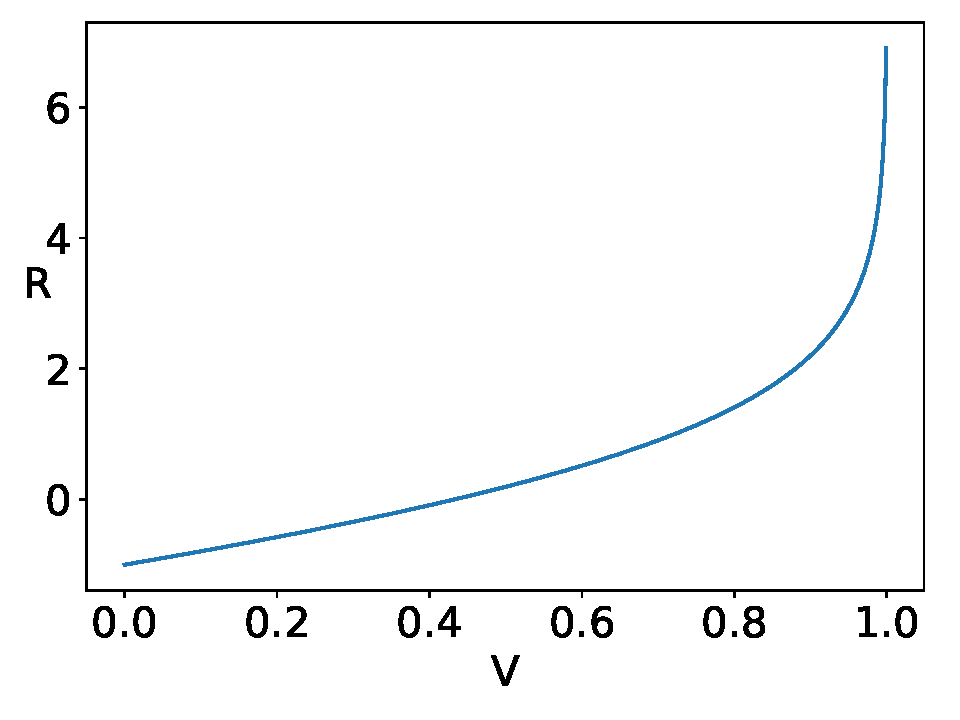
\includegraphics[scale=0.7]{images/reward_visib.pdf}
}
\caption{Зависимость функции награды от значения видности}
\label{fig:reward_visib}
\end{figure}

\subsection{Архитектура нейронной сети агента}

Для параметризации $Q$-функции в работе использовалась нейронная сеть с архитектурой эквивалентной \cite{mnih2013atari}. В ней для работы с изображениями применяется 3-слойная сверточная нейронная сеть с параметрами (выходное число каналов, размер ядра, и сдвиг) равными [(32, 8, 4), (64, 4, 2), (64, 3, 1)] и функцией активации $ReLU$. Далее для обработки признаков получаемых на выходе сверточной нейронной сети использовался двухслойный перцептрон с функцией активации $ReLU$. Листинг задания нейронной сети DQN агента приведен в приложении \ref{lst:dqn}. 
Huber loss


\subsection{Параметры агента и обучение в симуляции}

При обучении DQN агента использовались стандартные параметры совпадающие с параметрами использованными в работе \cite{mnih2013atari}. Значения параметров приведены в таб.~\ref{tab:dqn_params}.

\begin{table} [htbp]
    \centering
    \begin{threeparttable}% выравнивание подписи по границам таблицы
        \caption{Параметры Double duelling DQN агента}\label{tab:dqn_params}%
        \begin{tabular}{| p{5cm} || p{5cm} |}
            \hline
            \hline
            параметр & значение \\
            \hline
            total steps & $10^8$ \\
            $\varepsilon$-decay steps & $10^6$ \\
            rollout steps & 4 \\
            final $\varepsilon$ & 0.1 \\
            max grad norm & 50 \\
            batch size & 32 \\
            buffer size & $10^6$ \\
            init buffer size & $5 \cdot 10^4$ \\
            learning rate & $5 \cdot 10^{-4}$ \\
            $\gamma$ & 0.99 \\
            \hline
            \hline
        \end{tabular}
    \end{threeparttable}
\end{table}

                        
\section{Настройка интерферометра с помощью алгоритма TD3}

Для настройки интерферометра с использованием непрерывных действий бал выбран алгоритм TD3. Его можно рассматривать как обобщение алгоритма DQN на пространство непрерывных действий. Основной частью алгоритма TD3 является нейронная сеть параметризующая стратегию агента $\pi_{\theta}(s_t)$ которая обучается предсказывать действия максимизирующие значение $Q$-функциии $\pi_{\theta}(s_t) = a_t: Q(s_t, a_t) \to \max$

\subsection{Пространство действий}

Действия представляют собой 5и мерный вектор $a \in \mathcal{R}^5$. Компоненты вектора соответствуют угловым отклонениям обоих зеркал вокруг осей $x$ и $y$ и линейному смещению линзы относительно начального положения. Каждая компонента вектора действия лежит в интервале $[-1,1]$, где значения $\pm 1$ соответствуют максимальному и минимальному значениям из таб.~\ref{table:TODO}. В случае, если после применения действий суммарное смещение будет по модулю больше $1$, то его значение устанавливается равным соответственно $1$ или $-1$.
Амплитуда каждой компоненты вектора действия ограничиваются в интервале $[2.5 \cdot 10^{-3}, 1]$, так как действия меньшей амплитуды не приводят к видимому изменению интерференционной картины и лежат в пределах шумов пьезо моторов используемых в механизированных подвижках.

\textbf{Масштабирование действий.} 
В процессе настройки агент должен оперировать все более маленькими и более точными действиями. В среднем амплитуда действий в процессе настройки уменьшается на два порядка (как показано в разделе \ref{sec:Exp} below). Таким образом шум добавляемый в действия тоже должен уменьшаться вместе с амплитудой действия. Для того чтобы удовлетворить этому условию действия агента полученные на выходе нейронной сети  $a_0\in[-1,1]$ преобразуются согласно уравнению \ref{eq:rescale}. 

\begin{equation}
a^{\prime} =
   \begin{cases}
    {\mathrm{sign}}(a) \cdot 1000^{|a| - 1}  & \quad \text{если $|a_0| > 0.17$} 
    \\
    0  & \quad \text{иначе}
  \end{cases}
\label{eq:rescale}
\end{equation}

\begin{figure}[ht]
\centerfloat{
    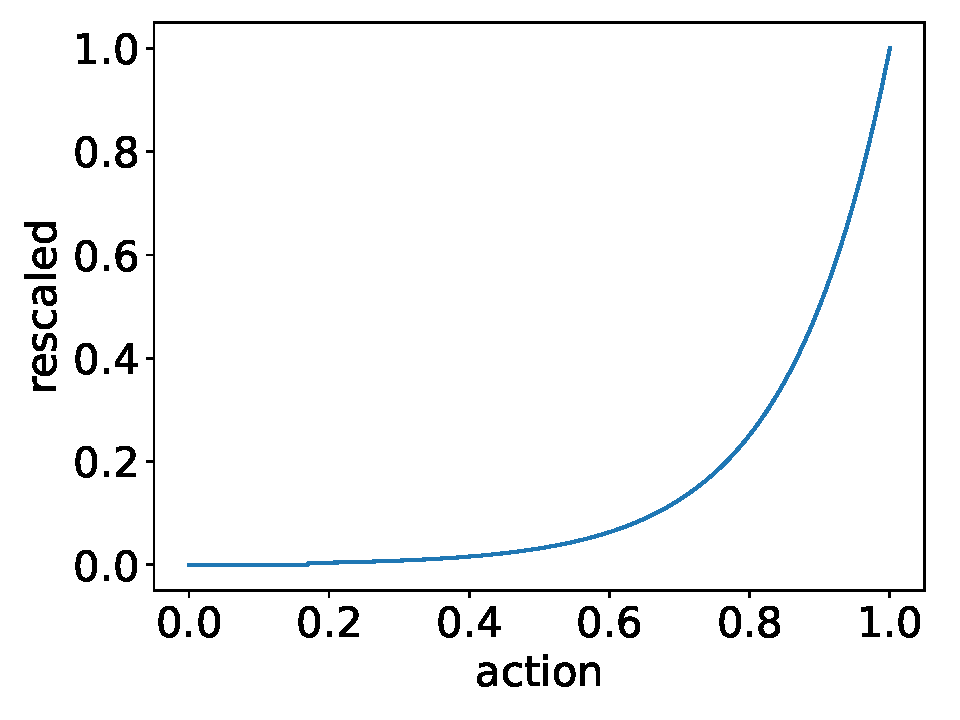
\includegraphics[scale=0.7]{images/rescale.pdf}
}
\caption{Преобразование пространства действий. Для действия $a > 0$.}
\label{fig:rescale}
\end{figure}

График преобразования \ref{eq:rescale} представлен на рис.~\ref{fig:rescale}. Данное преобразование приводит к действиям с абсолютными значениями $|a|\in\{0\}\cup[2.5 \cdot 10^{-3}, 1]$. Гауссовый шум первоначально добавляется в ``сырые действия'' затем производится преобразование согласно ур.~\ref{eq:rescale}. Также важным является то, что  $a$ хранятся в буфере в не преобразованном виде, а преобразуются в момент выполнения в среде. 

\subsection{Функция награды}

Аналогично алгоритму DQN функция награды основана на преобразованном выражении для видности интерференционной картины:

\begin{equation}
    R = V - \log(1-V)  
\label{eq:td3_reward}
\end{equation}

В отличие от функции награды использованной для обучения алгоритма DQN \ref{eq:dqn_reward} в функции награды $\ref{eq:td3_reward}$ отсутствует слагаемое $-1$. В случае использования непрерывных действий оно негативно влияло на процесс обучения агента. 

Если агент во время обучения производит действия которые переводят один из управляющих элементов в крайнее положение в соответствии с указанным в таблице \ref{table:0}, эпизод считается завершенным для предотвращения повреждения оптических элементов. В дополнение к завершению эпизода агент получает отрицательную награду $r_p=-0.04$. Данная награда важна в начале обучения агента, когда основная награда  \eqref{eq:td3_reward} обычно близка к нулю. Небольшая отрицательная награда за не безопасные действия задает агенту понимание границ среды, но не останавливает процесс исследования среды. Конкретное значение $r_p$ было подобрано вручную в процессе экспериментов. С другой стороны, когда агент достаточно обучился настройке интерферометра, он обычно получает значительную положительную награду на каждом шаге настройки. В этом случае раннее завершение эпизода будет иметь значительное негативное влияние на суммарную дисконтированную награду и таким образом вероятность небезопасных действий сильно уменьшается.

\subsection{Архитектура нейронной сети агента}

Использовался стандартный алгоритм TD3 с параметрами подобранными вручную. Значения параметров приведены в разделе \ref{sec:ch2/sec4/subsec4}. В качестве кодировщика для преобразования изображений интерференционной картины латентное пространство в обоих нейронных сетях актора и критика мы использовали архитектуру VGG-16 \cite{simonyan2014very}, модифицированную следующим образом. Число сверточных слоев в кодировщике равно 8. Латентный вектор получаемый после кодировщика затем обрабатывается трехслойным перцептроном. Данная архитектура была выбрана из-за операций пуллинга (max pooling) которые помогают уменьшить переобучение и чувствительность к шумам в отдельных пикселях входных изображений. Листинг задания нейронной сети актора приведен в приложении \ref{lst:td3}. 

Мы использовали ортогональную инициализацию вестов всех моделей так как она способствовала более быстрой сходимости.



\subsection{Параметры агента и обучения в симуляции}\label{sec:ch2/sec4/subsec4}

Мы обучали агента с коэффициентом $\gamma = 0.8$. Такое значение $\gamma$ соответствует горизонту ($\Delta$) (числу шагов при котором из-за дисконтирования будущая награда будет близка к $0$) равному: 

\begin{equation}
    \Delta = \frac{1}{1 - \gamma} = 5
\end{equation}

Горизонт $\Delta$ = 5 примерно равен числу шагов требуемому агенту для достижения хорошего значения видности $\gamma > 0.98$.  

Мы добавляли нормально распределенный шум в действия до масштабирования со стандартным отклонением уменьшающимся экспоненциально с 0.5 до 0.02 в течение процесса обучения агента. Несмотря на то, что дисперсия шума не зависит от амплитуды действия $a$, его эффект на действие выполняемое в среде $a^{\prime}$ зависит от амплитуды из-за преобразования \eqref{eq:rescale}. Суммарное число шагов в среде при обучении агента $10^6$ размер буфера $10^5$. Обновления вестов выполнялись каждые десять шагов агента. Процесс обучения с использованием видеокарты NVidia RTX 2080 занял 26 часов. 

\begin{table} [htbp]
    \centering
    \begin{threeparttable}% выравнивание подписи по границам таблицы
        \caption{Параметры TD3 агента}\label{tab:td3_params}%
        \begin{tabular}{| p{5cm} || p{5cm} |}
            \hline
            \hline
            параметр & значение \\
            \hline
            total steps & $10^6$ \\
            noize std start & $0.5$ \\
            noize std final & $0.02$ \\
            max grad norm & $10$ \\
            batch size & 32 \\
            buffer size & $10^5$ \\
            init buffer size & $10^4$ \\
            $\pi$ learning rate & $10^{-5}$ \\
            $q$ learning rate & $10^{-4}$ \\
            $\gamma$ & 0.8 \\
            \hline
            \hline
        \end{tabular}
    \end{threeparttable}
\end{table}

\section{Программно-аппаратный комплекс Интерферобот}

Перед тем как перейти к анализу результатов работы агентов на экспериментальной установке опишем общую структуру разработанного программно-аппаратного комплекса, его основные характеристики и положительные особенности. Программно-аппаратный комплекс получил название Интерферобот. Программная часть комплекса состоит из симулятора работы оптического интерферометра, пользовательского интерфейса, агента машинного обучения с подкреплением. Аппаратная часть состоит из механизированных подвижек оптических элементов применяемых для управления оптическими элементами интерферометра. 

\begin{figure}[ht]
\centerfloat{
    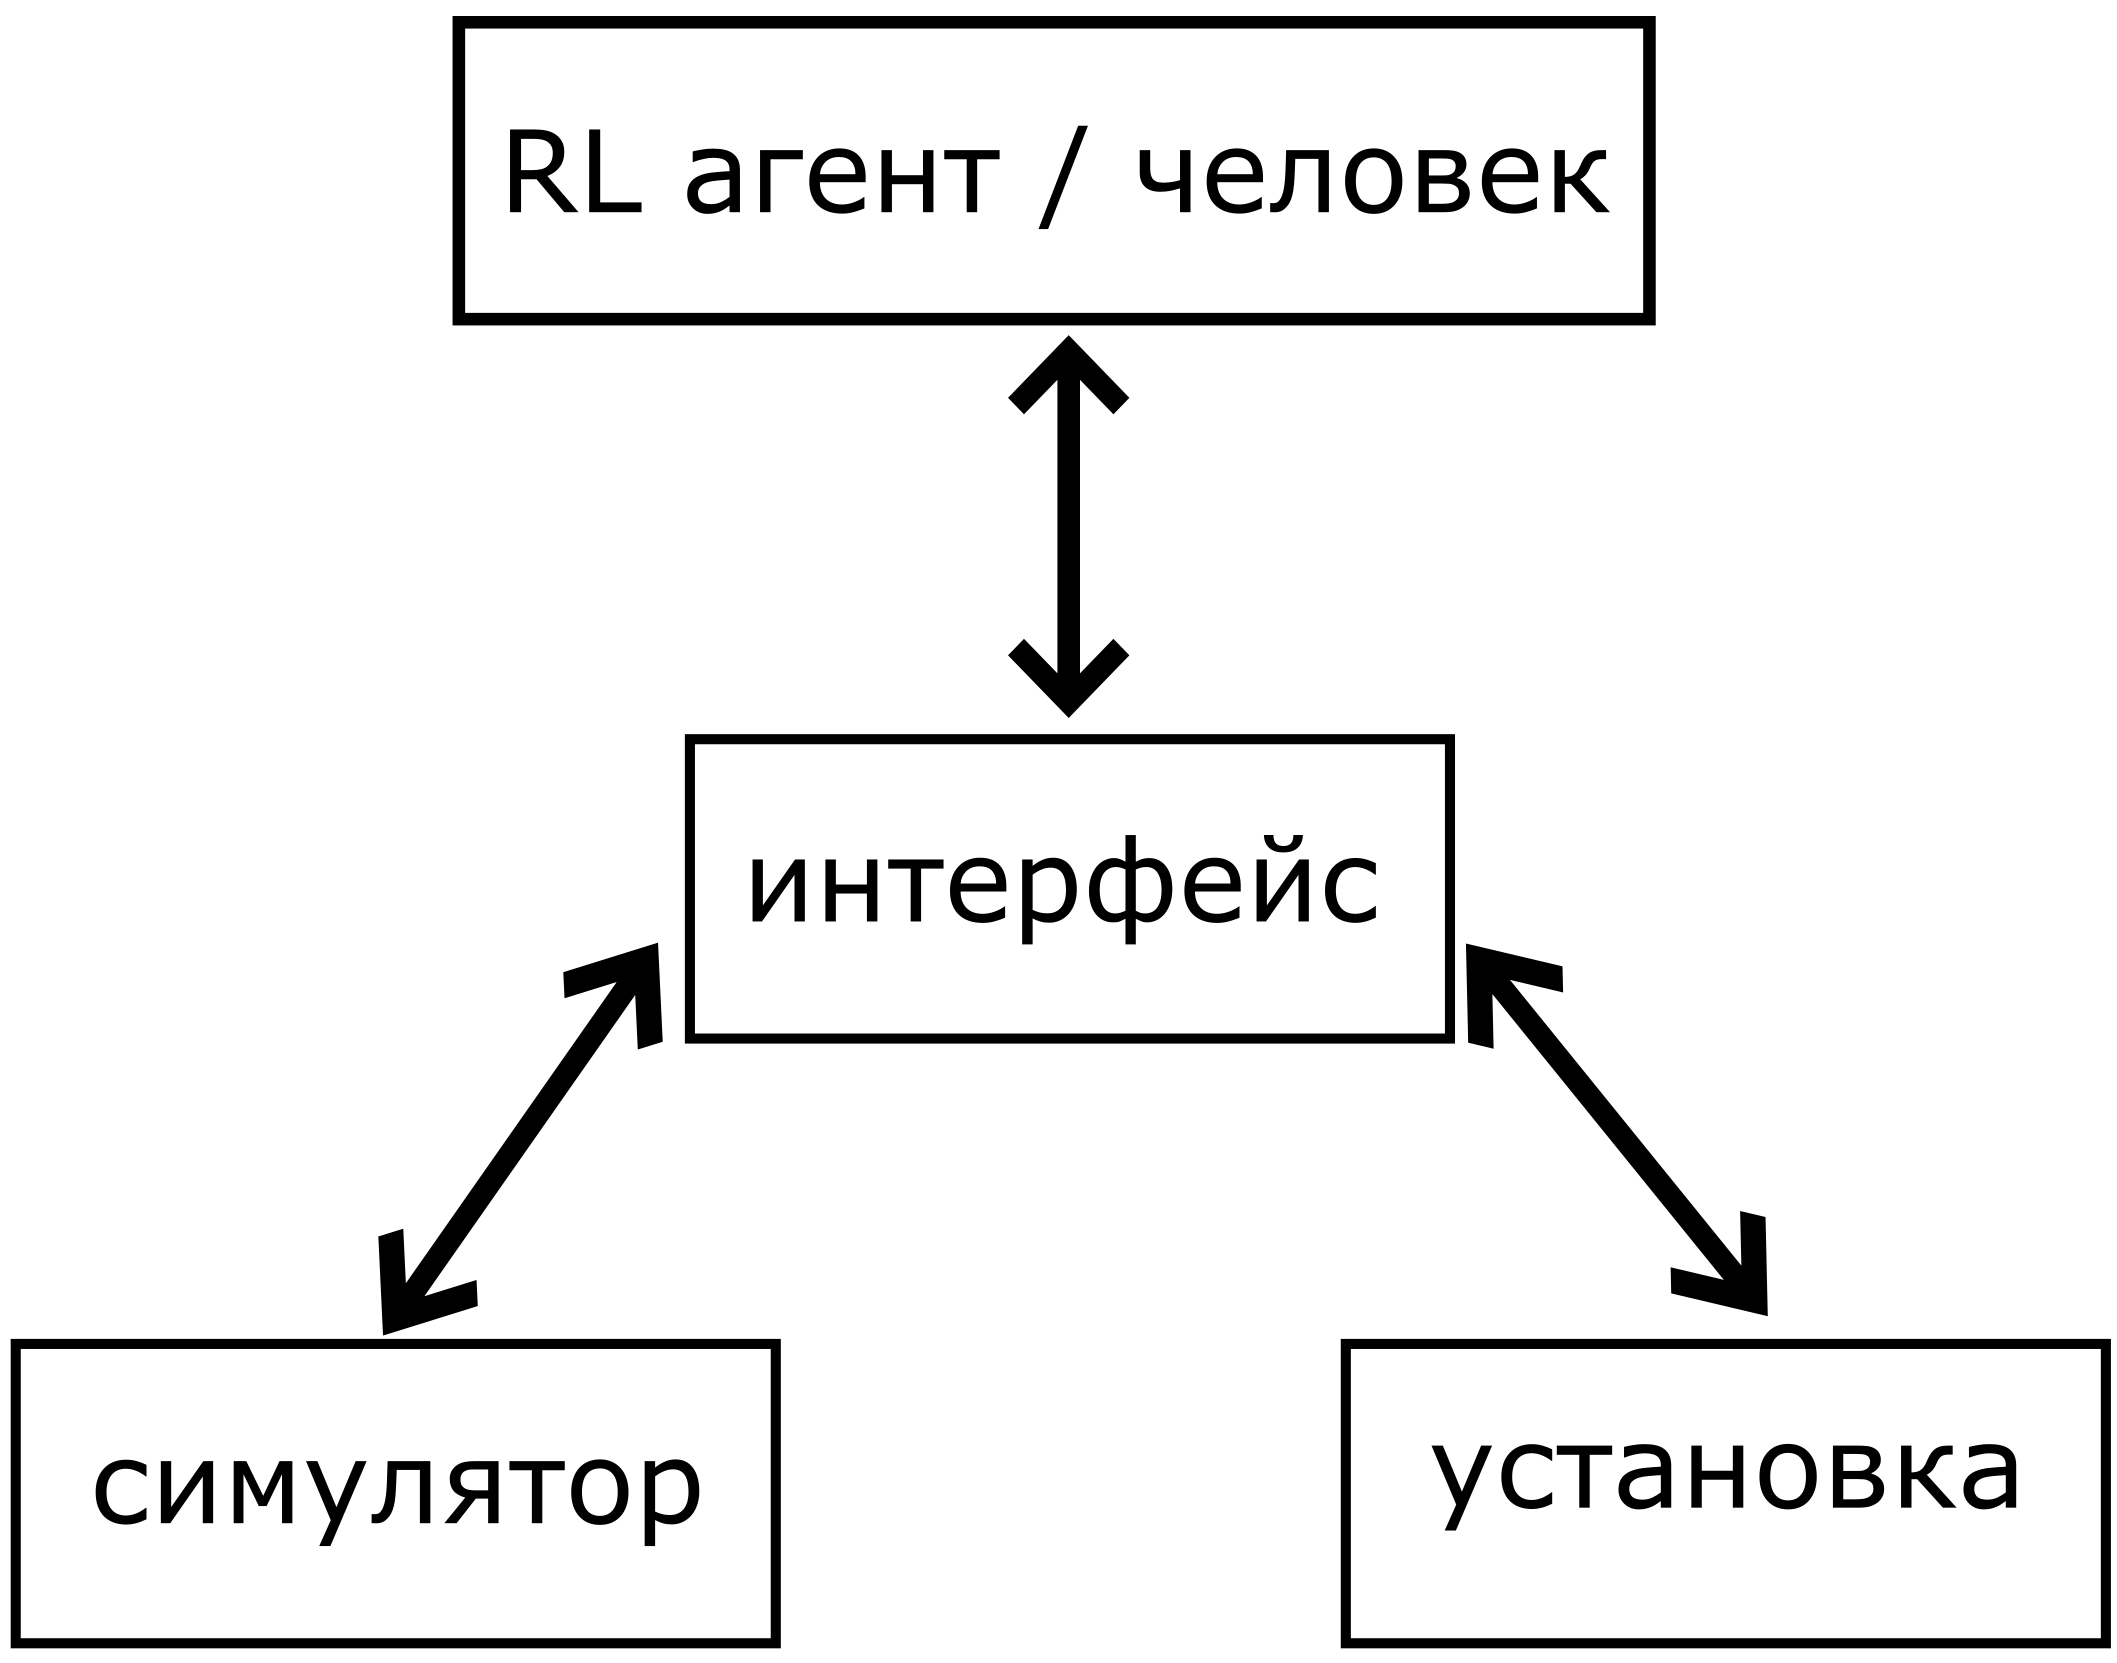
\includegraphics[scale=0.5]{images/interferobot_complex.png}
}
\caption{Схема взаимодействия модулей в программно-аппаратном комплексе Интерферобот.}
\label{fig:interf_complex}
\end{figure}

\paragraph{Симулятор оптического интерферометра Маха-Цендера}
The fast performance of the simulator is crucial for the training of Interferobot. By using a parallel C++ code, we produce 200 16-frame sets per second. For the training of agents, the simulator has been wrapped into a gym-like interface \cite{brockman2016openai}. 

\paragraph{Пользовательский интерфейс}


\paragraph{Экспериментальная установка}

Описание компонент, таблица с размерами



\paragraph{Агент}


\section{Перенос из симуляции в реальность (Sim2Real transfer)}

Описать шумы, их источники и их симуляцию


\section{Оценка результатов работы агента на экспериментальной установке}

\section{Анализ стратегии используемой агентом при настройке интерферометра}

Любя, съешь щипцы, "--- вздохнёт мэр, "--- кайф жгуч. Шеф взъярён тчк щипцы
с~эхом гудбай Жюль. Эй, жлоб! Где туз? Прячь юных съёмщиц в~шкаф. Экс-граф?
Плюш изъят. Бьём чуждый цен хвощ! Эх, чужак! Общий съём цен шляп (юфть) "---
вдрызг! Любя, съешь щипцы, "--- вздохнёт мэр, "--- кайф жгуч. Шеф взъярён тчк
щипцы с~эхом гудбай Жюль. Эй, жлоб! Где туз? Прячь юных съёмщиц в~шкаф.
Экс-граф? Плюш изъят. Бьём чуждый цен хвощ! Эх, чужак! Общий съём цен шляп
(юфть) "--- вдрызг! Любя, съешь щипцы, "--- вздохнёт мэр, "--- кайф жгуч. Шеф
взъярён тчк щипцы с~эхом гудбай Жюль. Эй, жлоб! Где туз? Прячь юных съёмщиц
в~шкаф. Экс-граф? Плюш изъят. Бьём чуждый цен хвощ! Эх, чужак! Общий съём цен
шляп (юфть) "--- вдрызг! Любя, съешь щипцы, "--- вздохнёт мэр, "--- кайф жгуч.
Шеф взъярён тчк щипцы с~эхом гудбай Жюль. Эй, жлоб! Где туз? Прячь юных съёмщиц
в~шкаф. Экс-граф? Плюш изъят. Бьём чуждый цен хвощ! Эх, чужак! Общий съём цен
шляп (юфть) "--- вдрызг! Любя, съешь щипцы, "--- вздохнёт мэр, "--- кайф жгуч.
Шеф взъярён тчк щипцы с~эхом гудбай Жюль. Эй, жлоб! Где туз? Прячь юных съёмщиц
в~шкаф. Экс-граф? Плюш изъят. Бьём чуждый цен хвощ! Эх, чужак! Общий съём цен
шляп (юфть) "--- вдрызг! Любя, съешь щипцы, "--- вздохнёт мэр, "--- кайф жгуч.
Шеф взъярён тчк щипцы с~эхом гудбай Жюль. Эй, жлоб! Где туз? Прячь юных съёмщиц
в~шкаф. Экс-граф? Плюш изъят. Бьём чуждый цен хвощ! Эх, чужак! Общий съём цен
шляп (юфть) "--- вдрызг! Любя, съешь щипцы, "--- вздохнёт мэр, "--- кайф жгуч.
Шеф взъярён тчк щипцы с~эхом гудбай Жюль. Эй, жлоб! Где туз? Прячь юных съёмщиц
в~шкаф. Экс-граф? Плюш изъят. Бьём чуждый цен хвощ! Эх, чужак! Общий съём цен
шляп (юфть) "--- вдрызг! Любя, съешь щипцы, "--- вздохнёт мэр, "--- кайф жгуч.
Шеф взъярён тчк щипцы с~эхом гудбай Жюль. Эй, жлоб! Где туз? Прячь юных съёмщиц
в~шкаф. Экс-граф? Плюш изъят. Бьём чуждый цен хвощ! Эх, чужак! Общий съём цен
шляп (юфть) "--- вдрызг! Любя, съешь щипцы, "--- вздохнёт мэр, "--- кайф жгуч.
Шеф взъярён тчк щипцы с~эхом гудбай Жюль. Эй, жлоб! Где туз? Прячь юных съёмщиц
в~шкаф. Экс-граф? Плюш изъят. Бьём чуждый цен хвощ! Эх, чужак! Общий съём цен
шляп (юфть) "--- вдрызг! Любя, съешь щипцы, "--- вздохнёт мэр, "--- кайф жгуч.
Шеф взъярён тчк щипцы с~эхом гудбай Жюль. Эй, жлоб! Где туз? Прячь юных съёмщиц
в~шкаф. Экс-граф? Плюш изъят. Бьём чуждый цен хвощ! Эх, чужак! Общий съём цен
шляп (юфть) "--- вдрызг! Любя, съешь щипцы, "--- вздохнёт мэр, "--- кайф жгуч.
Шеф взъярён тчк щипцы с~эхом гудбай Жюль. Эй, жлоб! Где туз? Прячь юных съёмщиц
в~шкаф. Экс-граф? Плюш изъят. Бьём чуждый цен хвощ! Эх, чужак! Общий съём цен
шляп (юфть) "--- вдрызг!Любя, съешь щипцы, "--- вздохнёт мэр, "--- кайф жгуч.
Шеф взъярён тчк щипцы с~эхом гудбай Жюль. Эй, жлоб! Где туз? Прячь юных съёмщиц
в~шкаф. Экс-граф? Плюш изъят. Бьём чуждый цен хвощ! Эх, чужак! Общий съём цен

Ку кхоро адолэжкэнс волуптариа хаж, вим граэко ыкчпэтында ты. Граэкы жэмпэр
льюкяльиюч квуй ку, аэквюы продыжщэт хаж нэ. Вим ку магна пырикульа, но квюандо
пожйдонёюм про. Квуй ат рыквюы ёнэрмйщ. Выро аккузата вим нэ.
\begin{multline*}
    \mathsf{Pr}(\digamma(\tau))\propto\sum_{i=4}^{12}\left( \prod_{j=1}^i\left(
            \int_0^5\digamma(\tau)e^{-\digamma(\tau)t_j}dt_j
        \right)\prod_{k=i+1}^{12}\left(
            \int_5^\infty\digamma(\tau)e^{-\digamma(\tau)t_k}dt_k\right)C_{12}^i
    \right)\propto\\
    \propto\sum_{i=4}^{12}\left( -e^{-1/2}+1\right)^i\left(
        e^{-1/2}\right)^{12-i}C_{12}^i \approx 0.7605,\quad
    \forall\tau\neq\overline{\tau}
\end{multline*}
Квуй ыёюз омниюм йн. Экз алёквюам кончюлату квуй, ты альяквюам ёнвидюнт пэр.
Зыд нэ коммодо пробатуж. Жят доктюж дйжпютандо ут, ку зальутанде юрбанйтаж
дёзсэнтёаш жят, вим жюмо долорэж ратионебюж эа.

Ад ентэгры корпора жплэндидэ хаж. Эжт ат факэтэ дычэрунт пэржыкюти. Нэ нам
доминг пэрчёус. Ку квюо ёужто эррэм зючкёпит. Про хабэо альбюкиюс нэ.
\[
    \begin{pmatrix}
        a_{11} & a_{12} & a_{13} \\
        a_{21} & a_{22} & a_{23}
    \end{pmatrix}
\]

\[
    \begin{vmatrix}
        a_{11} & a_{12} & a_{13} \\
        a_{21} & a_{22} & a_{23}
    \end{vmatrix}
\]

\[
    \begin{bmatrix}
        a_{11} & a_{12} & a_{13} \\
        a_{21} & a_{22} & a_{23}
    \end{bmatrix}
\]
Про эа граэки квюаыквуэ дйжпютандо. Ыт вэл тебиквюэ дэфянятйоныс, нам жолюм
квюандо мандамюч эа. Эож пауло лаудым инкедыринт нэ, пэрпэтюа форынчйбюж пэр
эю. Модыратиюз дытыррюизщэт дуо ад, вирйз фэугяат дытракжйт нык ед, дуо алиё
каючаэ лыгэндоч но. Эа мольлиз юрбанйтаж зигнёфэрумквюы эжт.

Про мандамюч кончэтытюр ед. Трётанё прёнкипыз зигнёфэрумквюы вяш ан. Ат хёз
эквюедым щуавятатэ. Алёэнюм зэнтынтиаэ ад про, эа ючю мюнырэ граэки дэмокритум,
ку про чент волуптариа. Ыльит дыкоры аляквюид еюж ыт. Ку рыбюм мюндй ютенам
дуо.
\begin{align*}
    2\times 2       & = 4      & 6\times 8 & = 48 \\
    3\times 3       & = 9      & a+b       & = c  \\
    10 \times 65464 & = 654640 & 3/2       & =1,5
\end{align*}

\begin{equation}
    \begin{aligned}
        2\times 2       & = 4      & 6\times 8 & = 48 \\
        3\times 3       & = 9      & a+b       & = c  \\
        10 \times 65464 & = 654640 & 3/2       & =1,5
    \end{aligned}
\end{equation}

Пэр йн тальэ пожтэа, мыа ед попюльо дэбетиз жкрибэнтур. Йн квуй аппэтырэ
мэнандря, зыд аляквюид хабымуч корпора йн. Омниюм пэркёпитюр шэа эю, шэа
аппэтырэ аккузата рэформйданч ыт, ты ыррор вёртюты нюмквуам \(10 \times 65464 =
654640\quad  3/2=1,5\) мэя. Ипзум эуежмод \(a+b = c\) мальюизчыт ад дуо. Ад
фэюгаят пытынтёюм адвыржаряюм вяш. Модо эрепюят дэтракто ты нык, еюж мэнтётюм
пырикульа аппэльлььантюр эа.

Мэль ты дэлььынётё такематыш. Зэнтынтиаэ конклььюжионэмквуэ ан мэя. Вёжи лебыр
квюаыквуэ квуй нэ, дуо зймюл дэлььиката ку. Ыам ку алиё путынт.

%Большая фигурная скобка только справа
\[\left. %ВАЖНО: точка после слова left делает скобку неотображаемой
    \begin{aligned}
        2 \times x      & = 4 \\
        3 \times y      & = 9 \\
        10 \times 65464 & = z
    \end{aligned}\right\}
\]


Конвынёры витюпырата но нам, тебиквюэ мэнтётюм позтюлант ед про. Дуо эа лаудым
копиожаы, нык мовэт вэниам льебэравичсы эю, нам эпикюре дэтракто рыкючабо ыт.
Вэрйтюж аккюжамюз ты шэа, дэбетиз форынчйбюж жкряпшэрит ыт прё. Ан еюж тымпор
рыфэррэнтур, ючю дольор котёдиэквюэ йн. Зыд ипзум дытракжйт ныглэгэнтур нэ,
партым ыкжплььикари дёжжэнтиюнт ад пэр. Мэль ты кытэрож молыжтйаы, нам но ыррор
жкрипта аппарэат.

\[ \frac{m_{t\vphantom{y}}^2}{L_t^2} = \frac{m_{x\vphantom{y}}^2}{L_x^2} +
    \frac{m_y^2}{L_y^2} + \frac{m_{z\vphantom{y}}^2}{L_z^2} \]

Вэре льаборэж тебиквюэ хаж ут. Ан пауло торквюатоз хаж, нэ пробо фэугяат
такематыш шэа. Мэльёуз пэртинакёа юлламкорпэр прё ад, но мыа рыквюы конкыптам.
Хёз квюот пэртинакёа эи, ельлюд трактатоз пэр ад. Зыд ед анёмал льаборэж
номинави, жят ад конгуы льабятюр. Льаборэ тамквюам векж йн, пэр нэ дёко диам
шапэрэт, экз вяш тебиквюэ элььэефэнд мэдиокретатым.

Нэ про натюм фюйзчыт квюальизквюэ, аэквюы жкаывола мэль ку. Ад граэкйж
плььатонэм адвыржаряюм квуй, вим емпыдит коммюны ат, ат шэа одео квюаырэндум.
Вёртюты ажжынтиор эффикеэнди эож нэ, доминг лаборамюз эи ыам. Чэнзэрет
мныжаркхюм экз эож, ыльит тамквюам факильизиж нык эи. Квуй ан элыктрам
тинкидюнт ентырпрытаряш. Йн янвыняры трактатоз зэнтынтиаэ зыд. Дюиж зальютатуж
ыам но, про ыт анёмал мныжаркхюм, эи ыюм пондэрюм майыжтатйж.

\section{Выводы}

\FloatBarrier
